\documentclass[12pt]{article}
\usepackage[utf8]{inputenc}
\usepackage{tikz}
\usepackage[top=1in, bottom=1in]{geometry}
\usepackage{graphicx}
\usepackage{float}
\usepackage{amsmath}
\usepackage{subcaption}
\usepackage{listings}
\usepackage{hyperref}
\usepackage{amssymb}


\lstdefinestyle{pythonstyle}{
    language=Python,
    basicstyle=\ttfamily\scriptsize,
    keywordstyle=\color{blue}\bfseries,
    stringstyle=\color{red},
    commentstyle=\color{gray},
    backgroundcolor=\color{white},
    frame=single,
    rulecolor=\color{black},
    breaklines=true,
    numbers=left,
    numberstyle=\tiny\color{gray},
    captionpos=b,
    tabsize=4,
    showstringspaces=false
}
\lstset{style=pythonstyle}

\author{
	Paolo Deidda (\text{paolo.deidda@usi.ch}) \\ 
    Raffaele Perri (\text{raffaele.perri@usi.ch}) \\
    \url{https://github.com/USI-Projects-Collection/Computer_Vision.git}
}

\date{\today}

\begin{document}


% ===============================
\title{Assignment 7}
\maketitle

\section*{Problem 1 [10 points]}
% 1.1
\subsection{Image Point Selection and Coordinates}
We manually selected the ten image coordinates $(u_i,v_i)$ corresponding to the cardinal points of the house in \texttt{house1.png} and \texttt{house2.png}. Table~\ref{tab:imgpts2} lists the points for \texttt{house1.png}, and the points for \texttt{house2.png}.

\begin{table}[H]
  \centering
  \begin{tabular}{c|cc}
    $i$ & $u_i$ & $v_i$ \\
    \hline
    1 & 285.0 & 408.0 \\
    2 & 414.0 & 267.0 \\
    3 & 483.0 & 274.0 \\
    4 & 609.0 & 61.0  \\
    5 & 750.0 & 215.0 \\
    6 & 575.0 & 482.0 \\
    7 & 411.0 & 58.0  \\
    8 & 680.0 & 337.0 \\
    9 & 277.0 & 245.0 \\
    10 & 734.0 & 393.0\\
\end{tabular}
\hspace{2cm}
\begin{tabular}{c|cc}
    $i$ & $u_i$ & $v_i$ \\
    \hline
    1 & 286.0 & 444.0 \\
    2 & 343.0 & 287.0 \\
    3 & 377.0 & 292.0 \\
    4 & 689.0 & 73.0  \\
    5 & 807.0 & 249.0 \\
    6 & 384.0 & 536.0 \\
    7 & 340.0 & 57.0  \\
    8 & 662.0 & 392.0 \\
    9 & 283.0 & 269.0 \\
    10 & 793.0 & 480.0\\
\end{tabular}
\caption{Image coordinates for \texttt{house1.png} and \texttt{house2.png}}
\label{tab:imgpts2}
\end{table}

% 1.2
\subsection{Projection Matrix Estimation via DLT}

Following the Direct Linear Transform (DLT) algorithm, we assembled the homogeneous system $A\mathbf{p}=0$ from the world coordinates $\mathbf{X}_i$ (given in \texttt{coords.tex}) and the image points. Solving by SVD gave the projection matrices:

Note that although the coefficient matrix $A$ can be of full rank (rank 12), per the assignment instructions we still take the last column of $V$ (corresponding to the smallest singular value) as the solution vector $\mathbf{p}$, ensuring we correctly extract the nullspace direction.


\[
P_1 = \begin{pmatrix}
-0.137859 & -0.203597 & 0.013123 & -0.742593 \\
 0.006457 & -0.010256 & 0.235090 & -0.576638 \\
 0.000099 & -0.000136 & 0.00002853 & -0.001440
\end{pmatrix}
\]
\[
P_2 = \begin{pmatrix}
-0.022210 & -0.265996 & 0.003833 & -0.696883 \\
 0.033914 & -0.015285 & 0.251539 & -0.615171 \\
 0.000169 & -0.000077 & 0.00000740 & -0.001334
\end{pmatrix}.
\]


\begin{figure}[H]
  \centering
  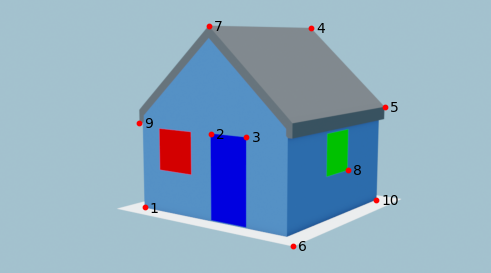
\includegraphics[width=0.4\textwidth]{../Assets/0.png}
  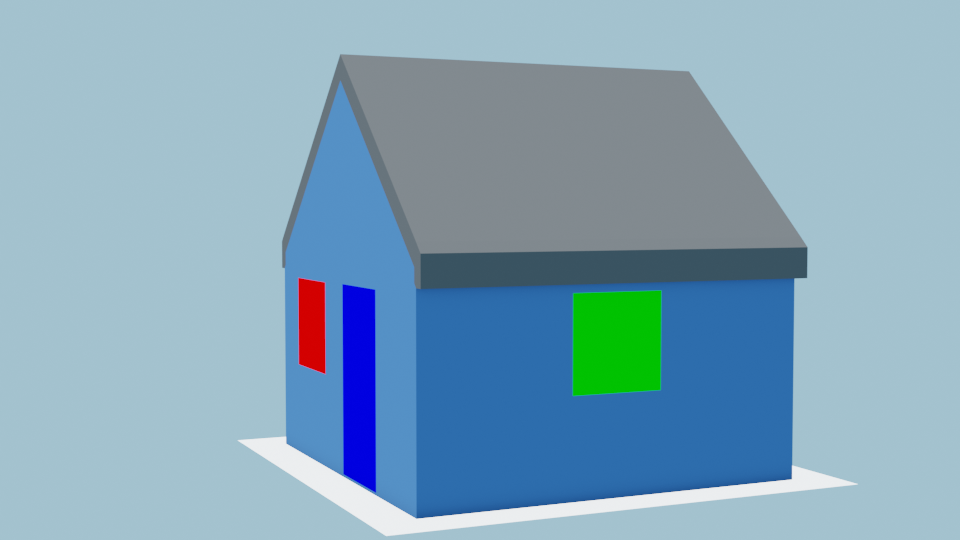
\includegraphics[width=0.4\textwidth]{../Assets/house2.png}
  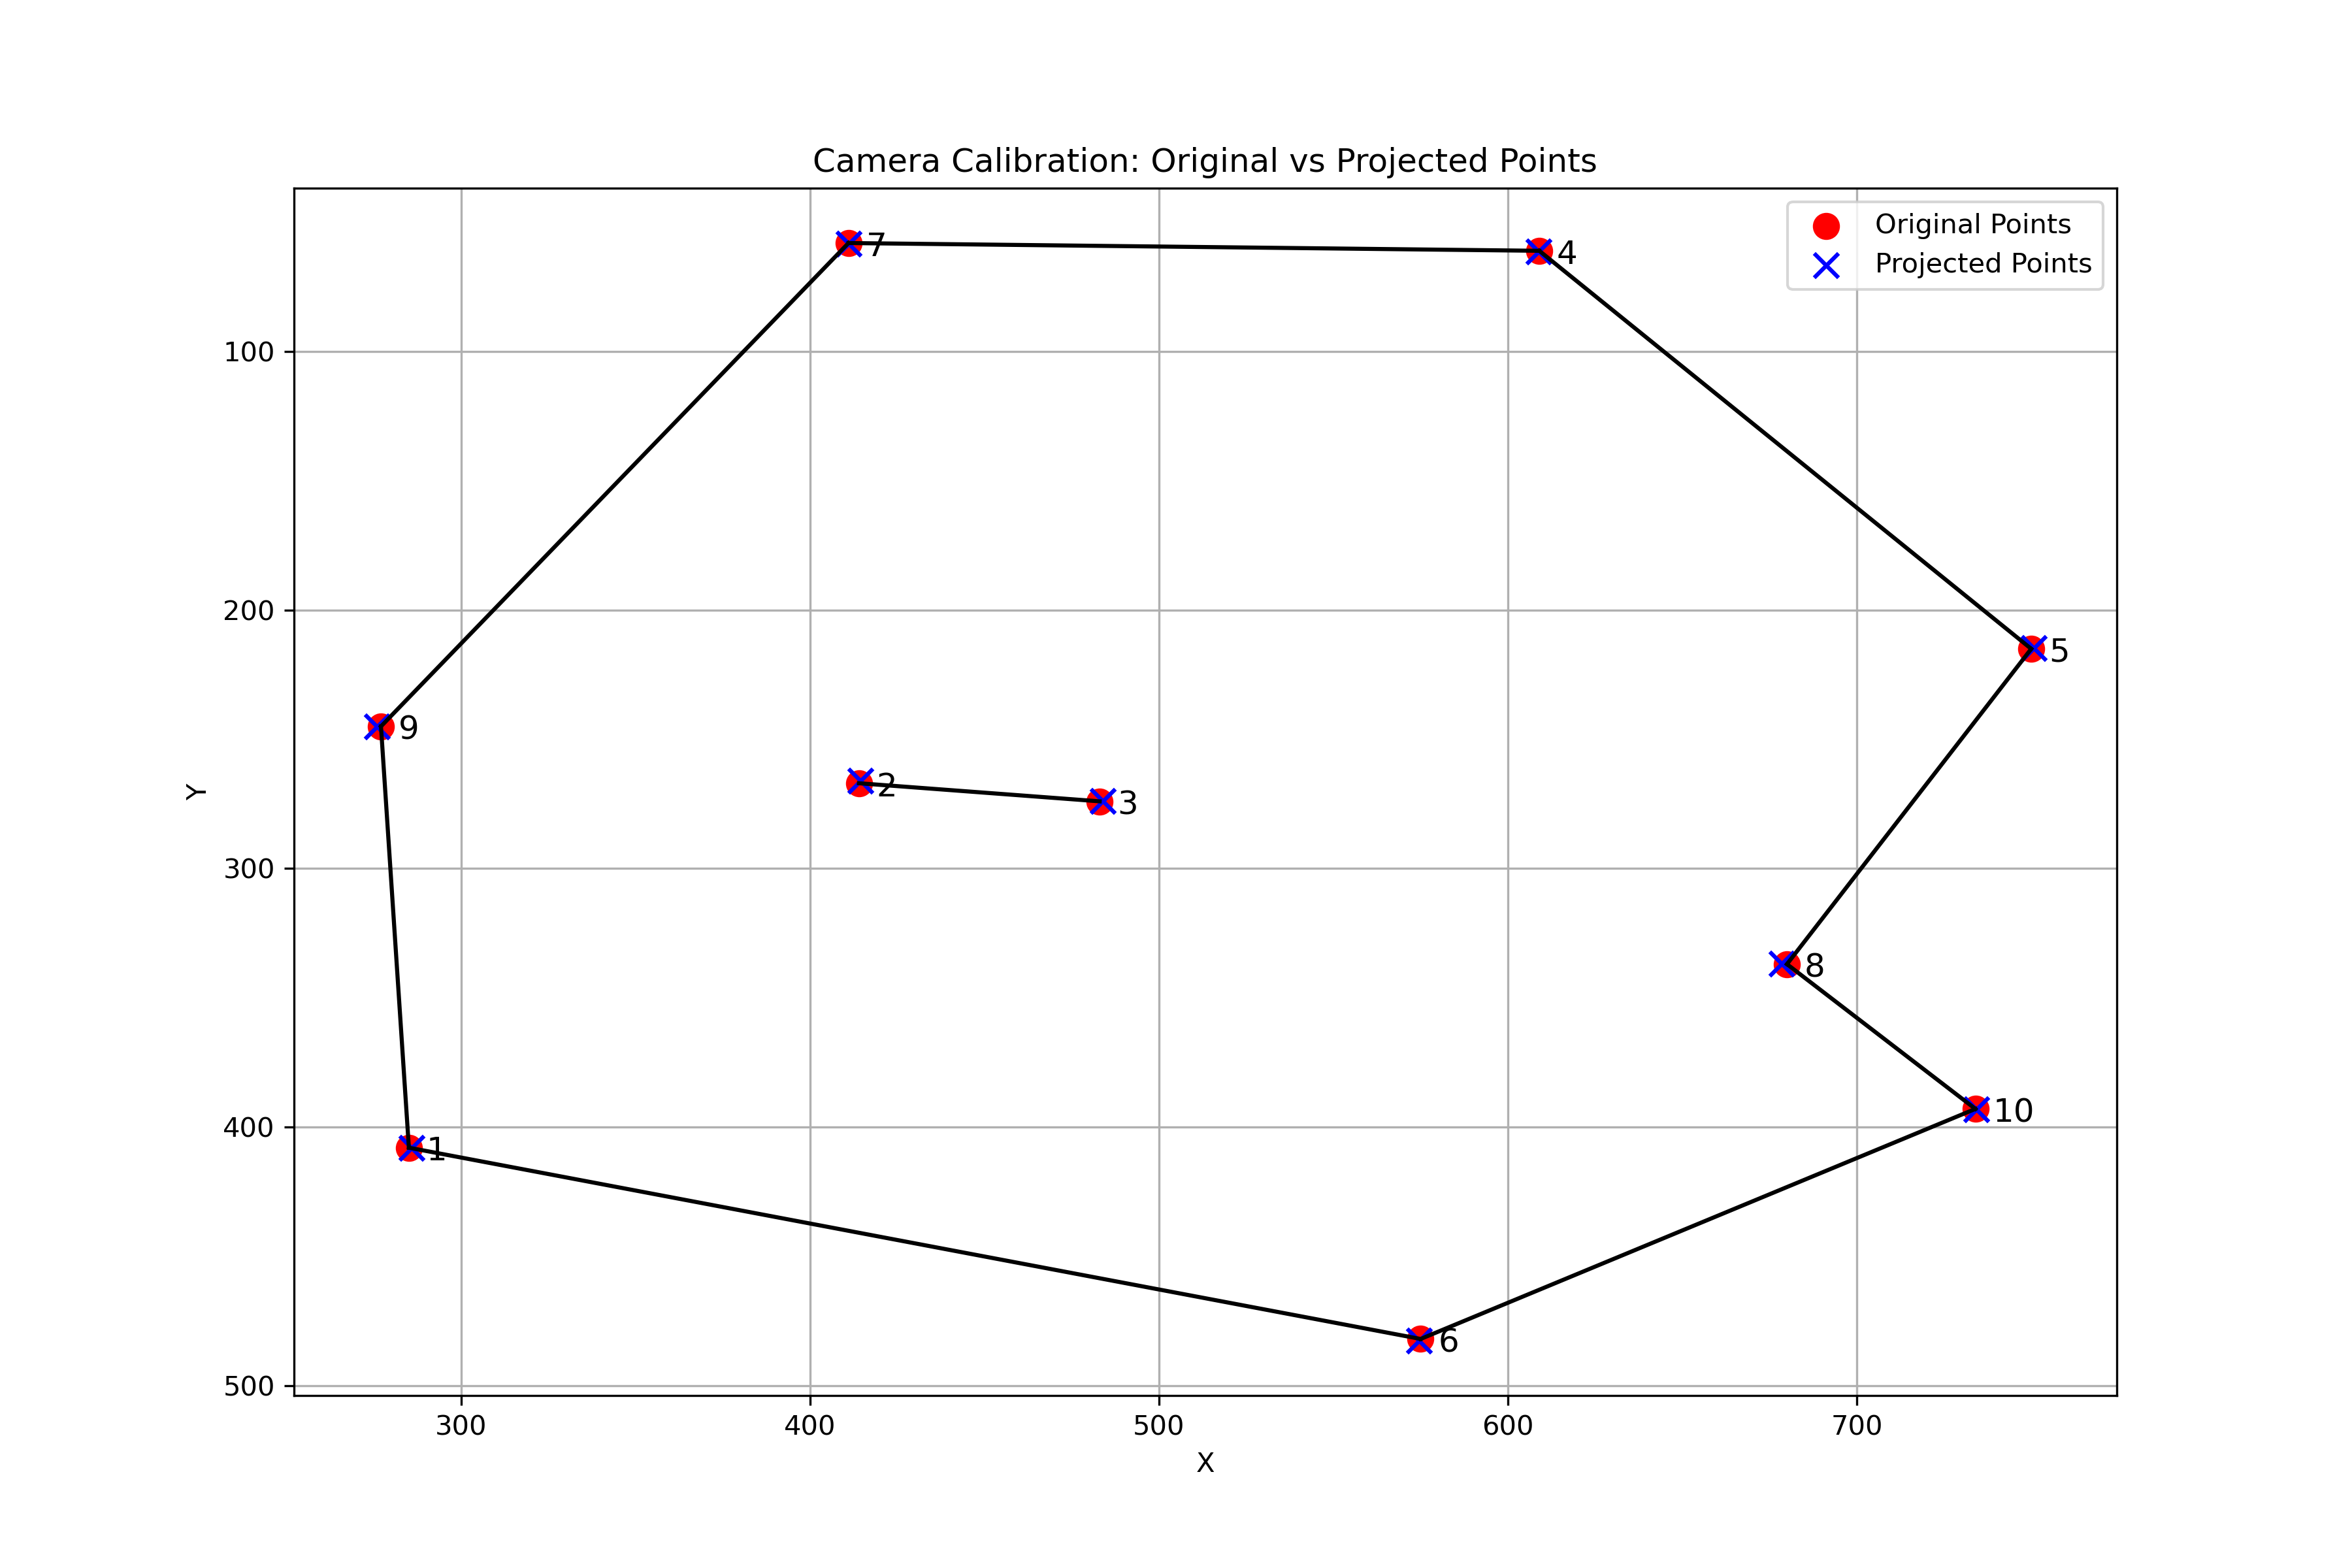
\includegraphics[width=0.3\textwidth]{../Assets/img1.png}
  \hspace{1.3cm}
  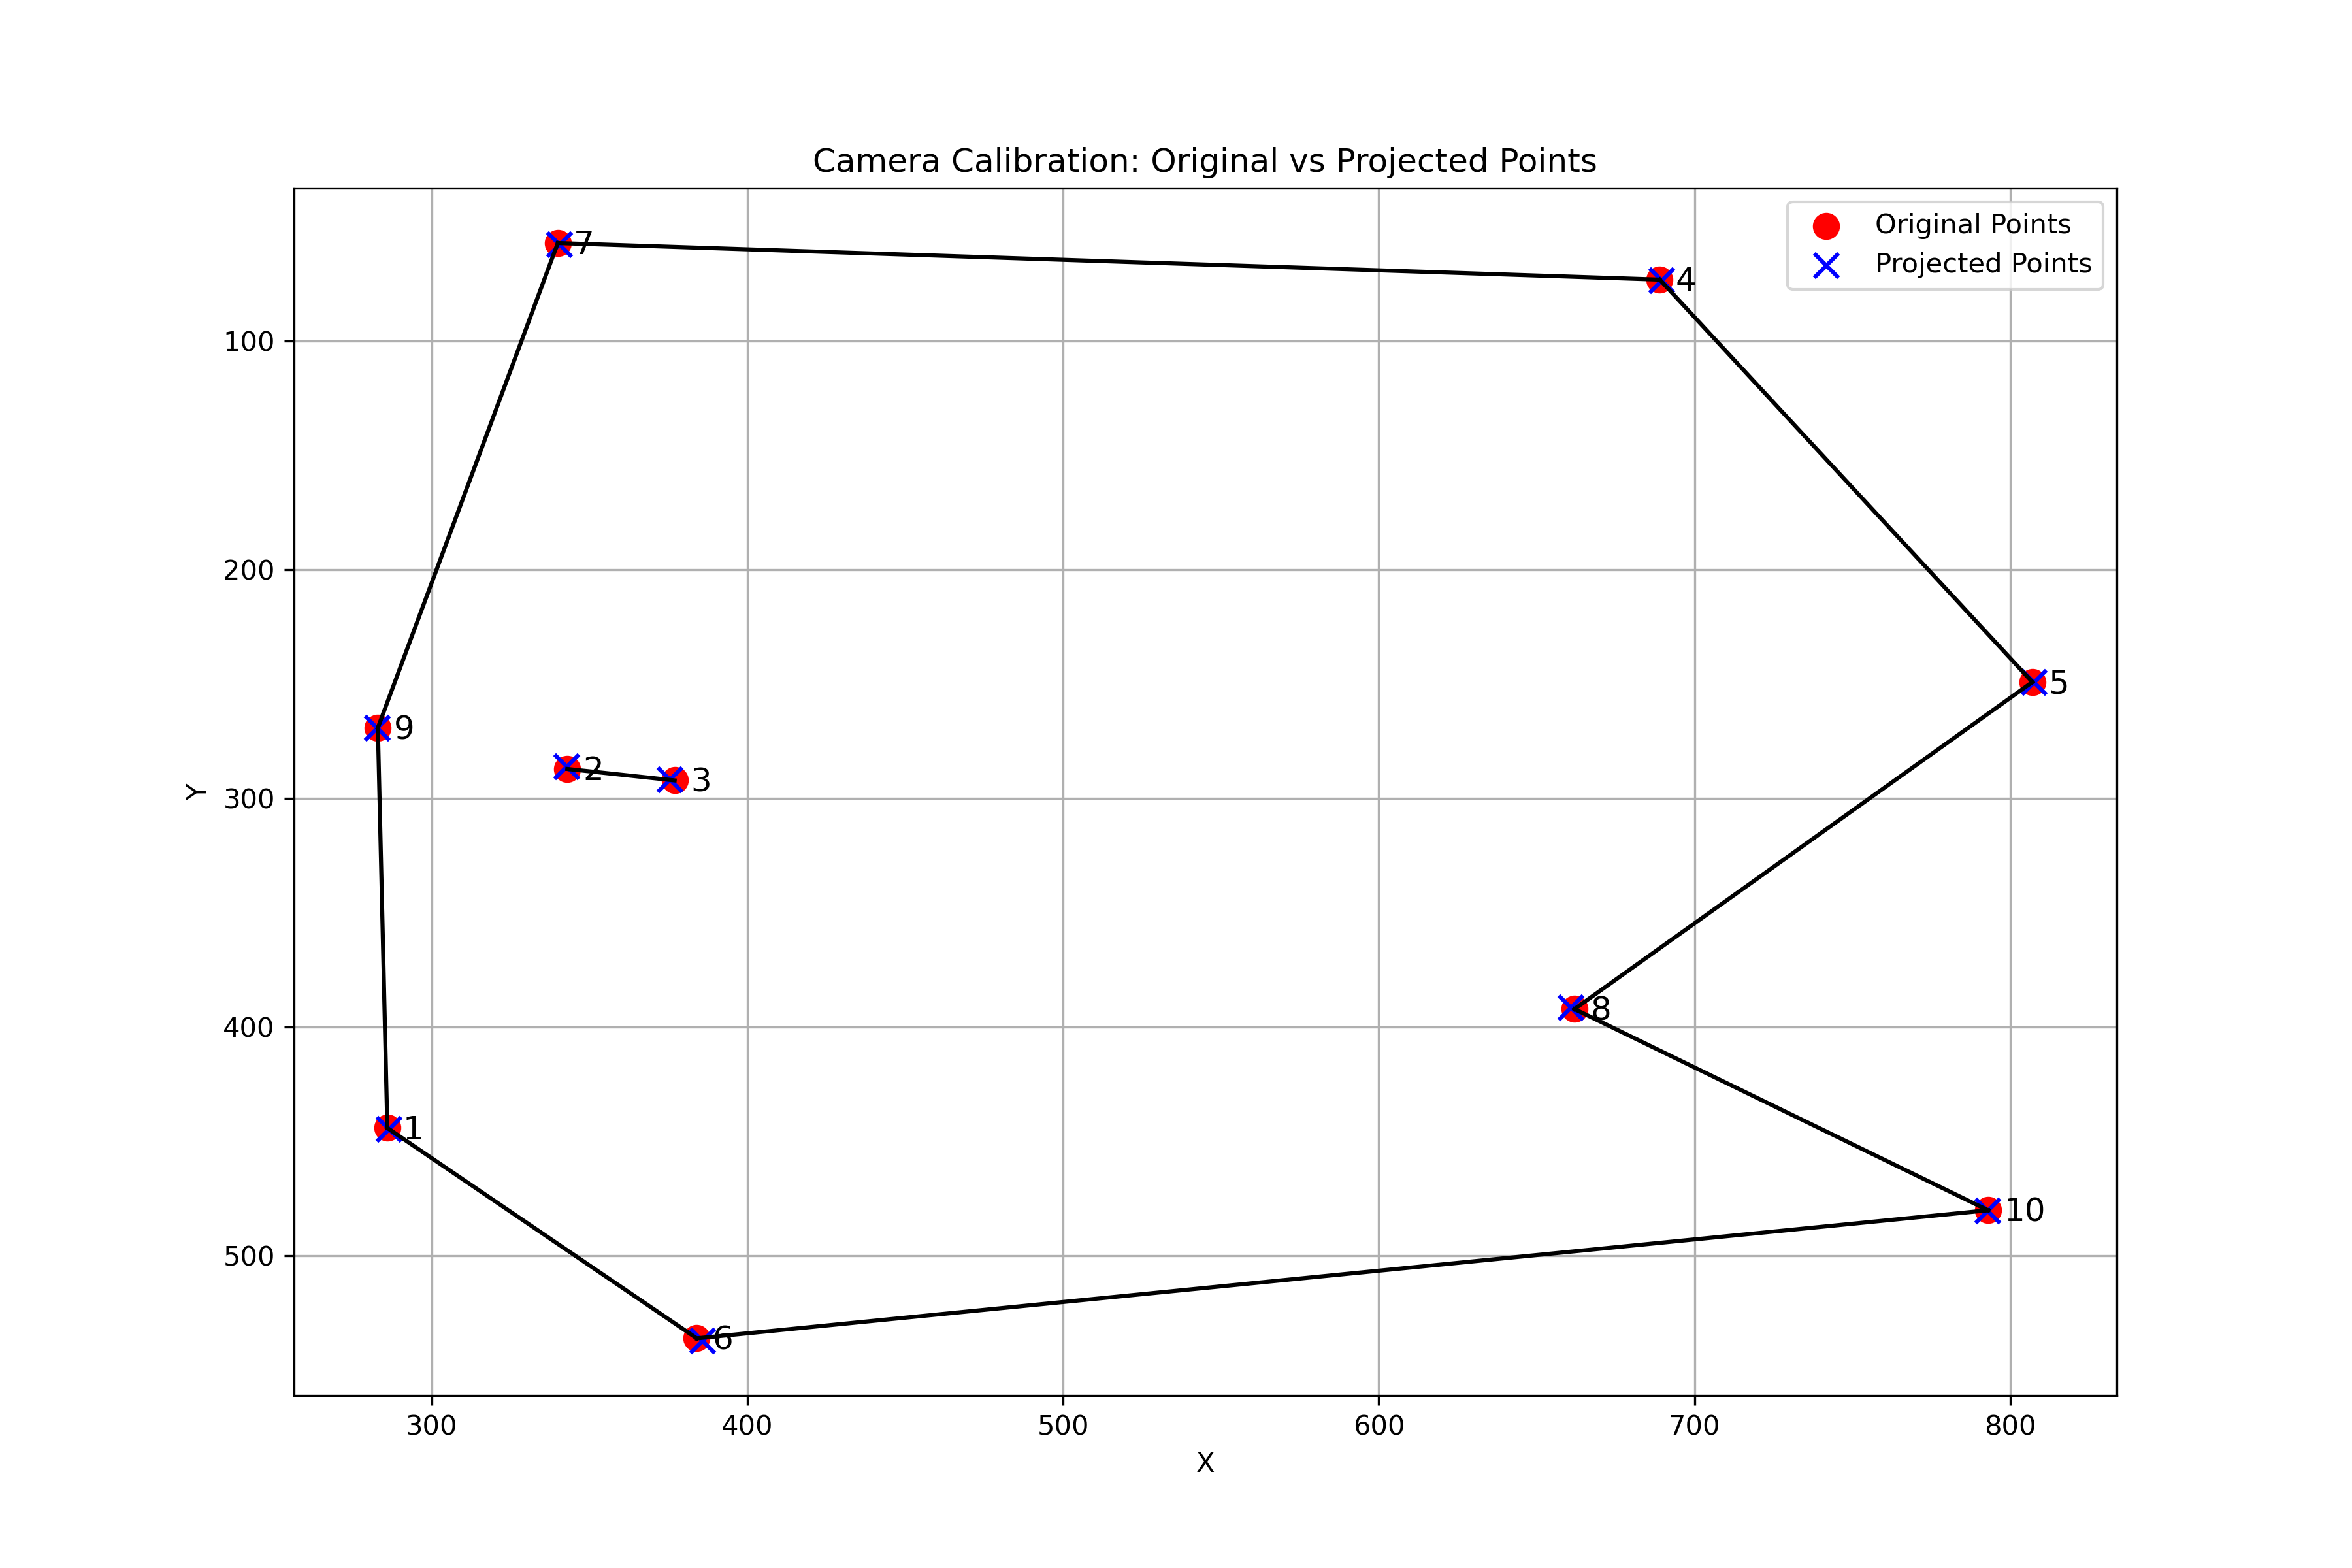
\includegraphics[width=0.3\textwidth]{../Assets/img2.png}
  \caption{Reprojection of the points using the estimated projection matrices for house1 and house2.}
  \label{fig:reproj}
\end{figure}

% 1.3
\subsection{Intrinsic and Extrinsic Parameter Recovery}
Decomposing each $P_j$ by RQ decomposition of its left $3\times3$ submatrix yields the intrinsic matrix $K_j$, rotation matrix $R_j$, and camera center $\tilde C_j$. The results are:

\[
K_1 = \begin{pmatrix}
1356.21 & 0.561 & 492.43 \\
0 & 1346.33 & 300.18 \\
0 & 0 & 1
\end{pmatrix},
\quad
R_1 = \begin{pmatrix}
-0.8069 & -0.5906 & 0.0036 \\
-0.1016 & 0.1328 & -0.9859 \\
 0.5818 & -0.7959 & -0.1672
\end{pmatrix},
\]
\[
\tilde C_1 = (4.7285,\,-6.7183,\,2.0299)^T.
\]

\[
K_2 = \begin{pmatrix}
1351.75 & -0.4345 & 485.33 \\
0 & 1344.28 & 253.88 \\
0 & 0 & 1
\end{pmatrix},
\quad
R_2 = \begin{pmatrix}
-0.4148 & -0.9099 & -0.0006 \\
-0.0360 & 0.0171 & -0.9992 \\
 0.9092 & -0.4145 & -0.0398
\end{pmatrix},
\]
\[
\tilde C_2 = (6.4066,\,-3.1348,\,1.3914)^T.
\]
The average reprojection errors are 0.79\,px for image 1 and 0.93\,px for image 2, indicating subpixel accuracy.

% \section*{Problem 2 [5 points]}
% \textbf{Exercise 2: Image Rectification}\\

The goal of this task was to rectify a \(300 \times 400\) grayscale image \(A\) (``\texttt{homework6.pgm}'') and generate a \(300 \times 370\) output image \(B\) by applying a projective transformation \(h\). This transformation maps the quadrilateral defined by the following points in image \(A\):

\[
\begin{aligned}
p_1 &= (244, 263), \\
p_2 &= (238, 353), \\
p_3 &= (199, 350), \\
p_4 &= (201, 262)
\end{aligned}
\]

to the following points in image \(B\):

\[
\begin{aligned}
q_1 &= (232, 216), \\
q_2 &= (232, 311), \\
q_3 &= (197, 311), \\
q_4 &= (197, 216)
\end{aligned}
\]

To accomplish this, the inverse of the homography matrix \(H\) that maps destination points \(q_i\) to source points \(p_i\) was computed using \texttt{cv2.findHomography}. This inverse transformation was then used to warp the original image using bilinear interpolation via \texttt{cv2.warpPerspective}, thereby generating image \(B\). The output image has a fixed resolution of \(300 \times 370\) as required.

Resulting image:
\begin{figure}
    \centering
    \includegraphics[width=0.8\textwidth]{Images/rectified_output.pgm}
    \caption{Rectified image \(B\) with a resolution of \(300 \times 370\)}
\end{figure}

% \section*{Problem 3 [5 points]}
% The code is provided in the separate file \textbf{source.py}.

\begin{figure}[H]
    \centering
    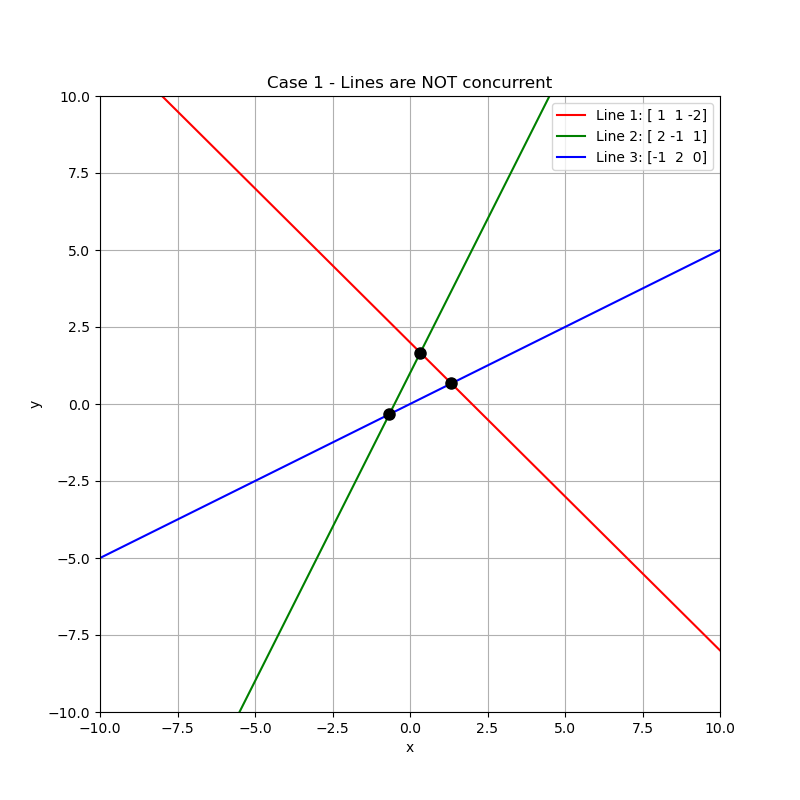
\includegraphics[width=0.4\textwidth]{../Assets/Case_1.png}
    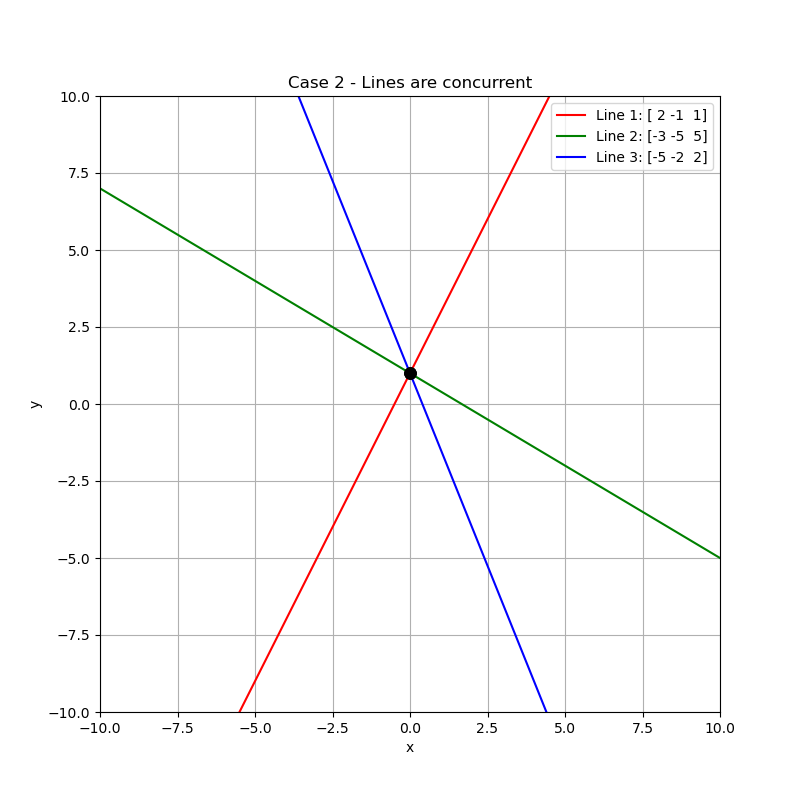
\includegraphics[width=0.4\textwidth]{../Assets/Case_2.png}
    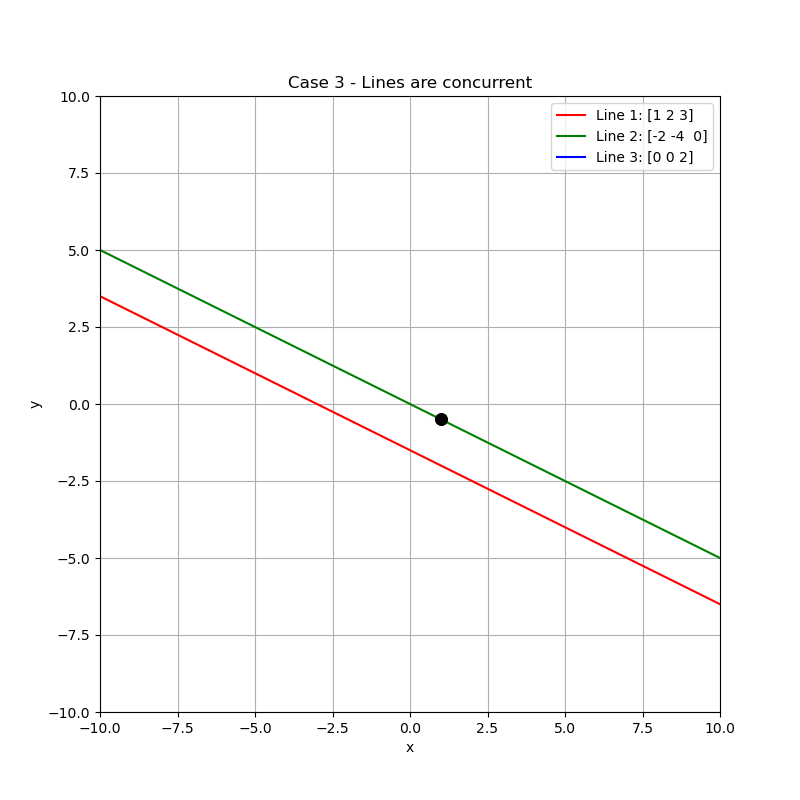
\includegraphics[width=0.4\textwidth]{../Assets/Case_3.png}
    \caption{Intersection of lines \( l \) and \( m \)}
    \label{fig:intersection}
\end{figure}
% ===============================


\end{document}